\providecommand{\qcor}[1]{\ulcorner#1\urcorner}   %

\section{笛卡尔函子}\label{sec:cartesian-functors}

我们现在来证明：\textbf{笛卡尔性}（cartesianness）是\trIsofibration{}的一条在%
\trEquivalence{}之下不变的性质；为此我们援引定理 5.2.8 来研究「见证一条%
\trIsofibration{}之笛卡尔性的数据」与「由一个\trEquivalence{}所提供的数据」%
这两者之间的关系。

\begin{corollary}\label{cor:equivalence-invariance}
考虑\trIsofibration{}之间的一个本质交换方块，其水平\trFunctor{}均为\trEquivalence：
\begin{center}
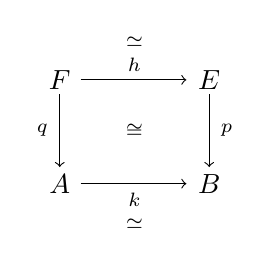
\begin{tikzpicture}[x=1.5em,y=1.5em]
  \node (F) at (0,1.5) {$F$};
  \node (E) at (3.6,1.5) {$E$};
  \node (A) at (0,-1.0) {$A$};
  \node (B) at (3.6,-1.0) {$B$};
  \draw[->] (0.5,1.5) -- (3.05,1.5);
  \node at (1.8,1.86) {$\scriptstyle h$};
  \node at (1.8,2.42) {$\scriptstyle\simeq$};
  \draw[->] (0,1.15) -- (0,-0.6);
  \node at (-0.42,0.28) {$\scriptstyle q$};
  \draw[->] (3.6,1.15) -- (3.6,-0.6);
  \node at (4.02,0.28) {$\scriptstyle p$};
  \node at (1.8,0.28) {$\scriptstyle\cong$};
  \draw[->] (0.5,-1.0) -- (3.05,-1.0);
  \node at (1.8,-1.4) {$\scriptstyle k$};
  \node at (1.8,-1.96) {$\scriptstyle\simeq$};
\end{tikzpicture}
\end{center}
则 $p$ 是一个\trCartesianFibration{}当且仅当 $q$ 是一个\trCartesianFibration；%
此时 $h$ 保持并反映笛卡尔变换：$\psi$ 是 $q$-\trCartesian，当且仅当 $h\psi$ 是%
$p$-\trCartesian。
\end{corollary}

\begin{proof}
由第 3 章中的\cref{prop:comma-weak-universal-property}，一个本质交换方块诱导一个%
本质交换方块
\begin{center}
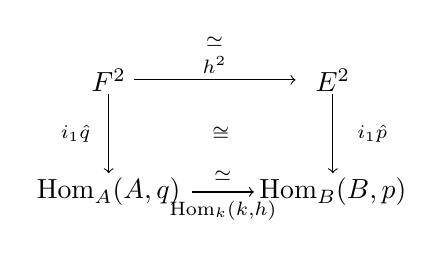
\begin{tikzpicture}[x=1.5em,y=1.5em]
  \node (F2) at (0,1.7) {$F^{2}$};
  \node (E2) at (5.4,1.7) {$E^{2}$};
  \node (HA) at (0,-1.0) {$\mathrm{Hom}_{A}(A,q)$};
  \node (HB) at (5.4,-1.0) {$\mathrm{Hom}_{B}(B,p)$};
  \draw[->] (0.6,1.7) -- (4.5,1.7);
  \node at (2.55,2.06) {$\scriptstyle h^{2}$};
  \node at (2.55,2.62) {$\scriptstyle\simeq$};
  \draw[->] (0,1.35) -- (0,-0.55);
  \node at (-0.8,0.4) {$\scriptstyle i_{1}\hat{q}$};
  \draw[->] (5.4,1.35) -- (5.4,-0.55);
  \node at (6.35,0.4) {$\scriptstyle i_{1}\hat{p}$};
  \node at (2.7,0.4) {$\scriptstyle\cong$};
  \draw[->] (2.0,-1.0) -- (3.5,-1.0);
  \node at (2.75,-0.6) {$\scriptstyle\simeq$};
  \node at (2.75,-1.44) {$\scriptstyle\mathrm{Hom}_{k}(k,h)$};
\end{tikzpicture}
\end{center}
其水平\trFunctor{}即为第 3 章中的\cref{prop:maps-between-commas}所定义的那些%
\trEquivalence。由伴随的等价不变性（见命题 B.3.8），左侧竖直\trFunctor{}容许一个%
右伴随右逆，当且仅当右侧竖直\trFunctor{}亦然。
由定理 5.2.8(ii) 即得：$p$ 是\trCartesian，当且仅当 $q$ 是\trCartesian。又由绝对%
右提升图表的等价不变性（见练习 2.3.vi 与 3.5.ii），类似地由%
\cref{thm:pcartesian-characterizations}(ii) 可知：$\psi$ 是 $q$-\trCartesian，%
当且仅当 $h\psi$ 是 $p$-\trCartesian。\footnote{原书印作「$\psi$ 是 $p$-笛卡尔的，%
当且仅当 $h\psi$ 是 $q$-笛卡尔的」，疑为 $p$、$q$ 互倒之误——$\psi$ 是 $F$ 中的%
变换，而 $p$ 定义在 $E$ 上，照录则不成类；此处径改。——译者注}
\end{proof}

迄今为止，我们已经遇到过\trCartesianFibration{}之间的几个保持结构的态射的例子。

\begin{definition}[笛卡尔函子]\label{def:cartesian-functor}
设 $p\colon E\twoheadrightarrow B$ 与 $q\colon F\twoheadrightarrow A$ 为%
\trCartesianFibration。一个交换方块定义了一个\textbf{笛卡尔函子}
（cartesian functor），若其定义域分量 $h$ 保持笛卡尔变换：若 $\psi$ 是%
$q$-\trCartesian，则 $h\psi$ 是 $p$-\trCartesian。
\begin{center}
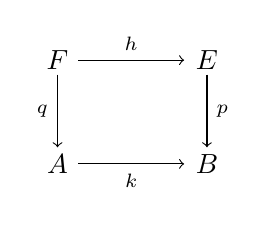
\begin{tikzpicture}[x=1.5em,y=1.5em]
  \node (F) at (0,1.5) {$F$};
  \node (E) at (3.6,1.5) {$E$};
  \node (A) at (0,-1.0) {$A$};
  \node (B) at (3.6,-1.0) {$B$};
  \draw[->] (0.5,1.5) -- node[above]{$\scriptstyle h$} (3.05,1.5);
  \draw[->] (0,1.15) -- node[left]{$\scriptstyle q$} (0,-0.6);
  \draw[->] (3.6,1.15) -- node[right]{$\scriptstyle p$} (3.6,-0.6);
  \draw[->] (0.5,-1.0) -- node[below]{$\scriptstyle k$} (3.05,-1.0);
\end{tikzpicture}
\end{center}
\end{definition}

为了第 6 章中的命题 6.3.14 之需，我们更愿意把这一术语保留给严格交换的方块；%
不过它也可以延拓到本质交换方块上。

\begin{example}[拉回与等价都是笛卡尔的]\label{exa:pullbacks-and-equivalences-cartesian}
直接由命题 5.2.4 与\cref{cor:equivalence-invariance}可知：拉回方块与由%
\trEquivalence{}构成的交换方块都定义笛卡尔函子；这些笛卡尔函子还带有如下特殊%
性质：其顶部水平\trFunctor{}既保持又反映笛卡尔变换。由于笛卡尔函子可以复合，%
这些结果可延拓至\trWeaklyCartesianSquare：任一\trWeaklyCartesianSquare{}都可%
分解为：
\begin{center}
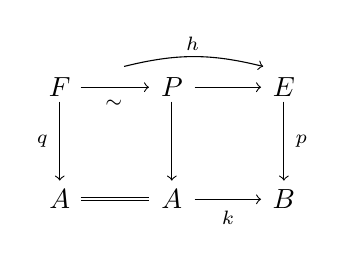
\begin{tikzpicture}[x=1.5em,y=1.5em]
  \node (F) at (0,1.7) {$F$};
  \node (P) at (2.7,1.7) {$P$};
  \node (E) at (5.4,1.7) {$E$};
  \node (A1) at (0,-1.0) {$A$};
  \node (A2) at (2.7,-1.0) {$A$};
  \node (B) at (5.4,-1.0) {$B$};
  \draw[->] (0.5,1.7) -- (2.15,1.7);
  \node at (1.3,1.3) {$\scriptstyle\sim$};
  \draw[->] (3.25,1.7) -- (4.85,1.7);
  \draw[->] (1.55,2.2) to[bend left=14] (4.9,2.2);
  \node at (3.2,2.75) {$\scriptstyle h$};
  \draw[->] (0,1.35) -- (0,-0.55);
  \node at (-0.42,0.4) {$\scriptstyle q$};
  \draw[->] (2.7,1.35) -- (2.7,-0.55);
  \node at (3.05,0.6) {$\scriptstyle\llcorner$};
  \draw[->] (5.4,1.35) -- (5.4,-0.55);
  \node at (5.82,0.4) {$\scriptstyle p$};
  \draw[double] (0.5,-1.0) -- (2.15,-1.0);
  \draw[->] (3.25,-1.0) -- (4.85,-1.0);
  \node at (4.05,-1.44) {$\scriptstyle k$};
\end{tikzpicture}
\end{center}
\end{example}

定理 5.2.8 对\trCartesianFibration{}的内部刻画可延拓为笛卡尔函子的一个内部刻画。

\begin{theorem}[笛卡尔函子的内部刻画]\label{thm:cartesian-functor-characterization}
对于\trCartesianFibration{}之间的一个交换方块
\begin{center}
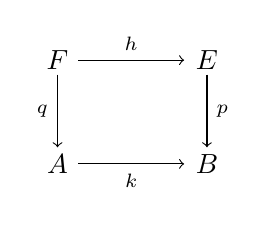
\begin{tikzpicture}[x=1.5em,y=1.5em]
  \node (F) at (0,1.5) {$F$};
  \node (E) at (3.6,1.5) {$E$};
  \node (A) at (0,-1.0) {$A$};
  \node (B) at (3.6,-1.0) {$B$};
  \draw[->] (0.5,1.5) -- node[above]{$\scriptstyle h$} (3.05,1.5);
  \draw[->] (0,1.15) -- node[left]{$\scriptstyle q$} (0,-0.6);
  \draw[->] (3.6,1.15) -- node[right]{$\scriptstyle p$} (3.6,-0.6);
  \draw[->] (0.5,-1.0) -- node[below]{$\scriptstyle k$} (3.05,-1.0);
\end{tikzpicture}
\end{center}
下列诸条等价：
\begin{enumerate}[label=(\roman*)]
\item 方块 $(h,k)$ 定义一个从 $q$ 到 $p$ 的笛卡尔函子。
\item 在左下方的函子图表中，恒同的\textbf{对应}（mate）是一个同构：
\begin{center}
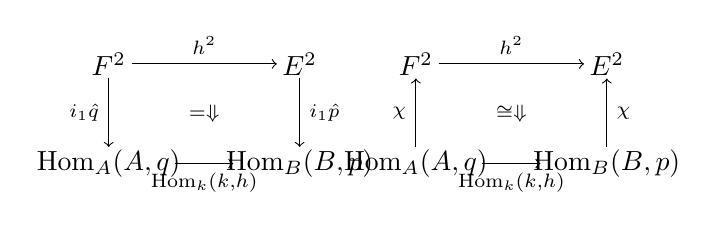
\begin{tikzpicture}[x=1.5em,y=1.5em]
  \node (F2) at (0,1.7) {$F^{2}$};
  \node (E2) at (4.6,1.7) {$E^{2}$};
  \node (HA) at (0,-0.7) {$\mathrm{Hom}_{A}(A,q)$};
  \node (HB) at (4.6,-0.7) {$\mathrm{Hom}_{B}(B,p)$};
  \draw[->] (0.55,1.7) -- node[above]{$\scriptstyle h^{2}$} (4.05,1.7);
  \draw[->] (0,1.35) -- node[left]{$\scriptstyle i_{1}\hat{q}$} (0,-0.3);
  \draw[->] (4.6,1.35) -- node[right]{$\scriptstyle i_{1}\hat{p}$} (4.6,-0.3);
  \draw[->] (1.6,-0.7) -- node[below]{$\scriptstyle\mathrm{Hom}_{k}(k,h)$} (3.0,-0.7);
  \node at (2.3,0.5) {$\scriptstyle=\Downarrow$};
  \node at (6.1,0.5) {$\scriptstyle\rightsquigarrow$};
  \begin{scope}[shift={(7.4,0)}]
  \node (F2b) at (0,1.7) {$F^{2}$};
  \node (E2b) at (4.6,1.7) {$E^{2}$};
  \node (HAb) at (0,-0.7) {$\mathrm{Hom}_{A}(A,q)$};
  \node (HBb) at (4.6,-0.7) {$\mathrm{Hom}_{B}(B,p)$};
  \draw[->] (0.55,1.7) -- node[above]{$\scriptstyle h^{2}$} (4.05,1.7);
  \draw[->] (0,-0.3) -- node[left]{$\scriptstyle\qcor{\chi}$} (0,1.35);
  \draw[->] (4.6,-0.3) -- node[right]{$\scriptstyle\qcor{\chi}$} (4.6,1.35);
  \draw[->] (1.6,-0.7) -- node[below]{$\scriptstyle\mathrm{Hom}_{k}(k,h)$} (3.0,-0.7);
  \node at (2.3,0.5) {$\scriptstyle\cong\Downarrow$};
  \end{scope}
\end{tikzpicture}
\end{center}
\item 在左下方位于 $k\colon A\to B$ 之上的函子图表中，恒同的对应是一个同构：
\begin{center}
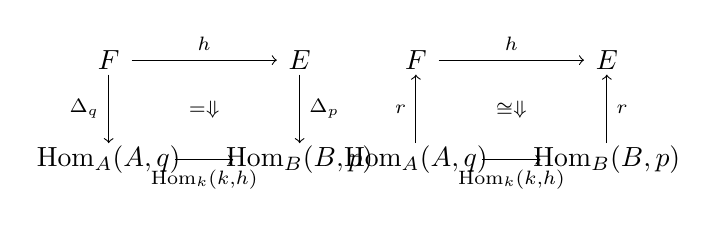
\begin{tikzpicture}[x=1.5em,y=1.5em]
  \node (F) at (0,1.7) {$F$};
  \node (E) at (4.6,1.7) {$E$};
  \node (HA) at (0,-0.7) {$\mathrm{Hom}_{A}(A,q)$};
  \node (HB) at (4.6,-0.7) {$\mathrm{Hom}_{B}(B,p)$};
  \draw[->] (0.55,1.7) -- node[above]{$\scriptstyle h$} (4.05,1.7);
  \draw[->] (0,1.35) -- node[left]{$\scriptstyle\Delta_{q}$} (0,-0.3);
  \draw[->] (4.6,1.35) -- node[right]{$\scriptstyle\Delta_{p}$} (4.6,-0.3);
  \draw[->] (1.6,-0.7) -- node[below]{$\scriptstyle\mathrm{Hom}_{k}(k,h)$} (3.0,-0.7);
  \node at (2.3,0.5) {$\scriptstyle=\Downarrow$};
  \node at (6.1,0.5) {$\scriptstyle\rightsquigarrow$};
  \begin{scope}[shift={(7.4,0)}]
  \node (Fb) at (0,1.7) {$F$};
  \node (Eb) at (4.6,1.7) {$E$};
  \node (HAb) at (0,-0.7) {$\mathrm{Hom}_{A}(A,q)$};
  \node (HBb) at (4.6,-0.7) {$\mathrm{Hom}_{B}(B,p)$};
  \draw[->] (0.55,1.7) -- node[above]{$\scriptstyle h$} (4.05,1.7);
  \draw[->] (0,-0.3) -- node[left]{$\scriptstyle r$} (0,1.35);
  \draw[->] (4.6,-0.3) -- node[right]{$\scriptstyle r$} (4.6,1.35);
  \draw[->] (1.6,-0.7) -- node[below]{$\scriptstyle\mathrm{Hom}_{k}(k,h)$} (3.0,-0.7);
  \node at (2.3,0.5) {$\scriptstyle\cong\Downarrow$};
  \end{scope}
\end{tikzpicture}
\end{center}
\end{enumerate}
\end{theorem}

此处所论的诸\emph{对应}推广了「伴随」或「转置」2-胞腔的概念（见附录 B 中的%
定义 B.3.3 与 B.3 节）。正如附录 B 中的警告 B.3.7 所注意到的，一个同构的对应%
未必可逆。

\begin{proof}
我们证明 (i)$\Leftrightarrow$(iii) 与 (i)$\Leftrightarrow$(ii)。为节省篇幅，我们以%
$\tilde{h}$ 作为函子 $\mathrm{Hom}_{k}(k,h)$ 的缩写。

\textbf{(i)$\Leftrightarrow$(ii)：}方块 $(h,k)$ 定义一个从 $q$ 到 $p$ 的笛卡尔函子，%
当且仅当它把泛 $q$-笛卡尔提升 $\qcor{\chi}\colon\mathrm{Hom}_{A}(A,q)\to F^{2}$ %
送到一支 $p$-笛卡尔箭头；换言之，当且仅当该交换图表定义出一个绝对右提升：
\begin{center}
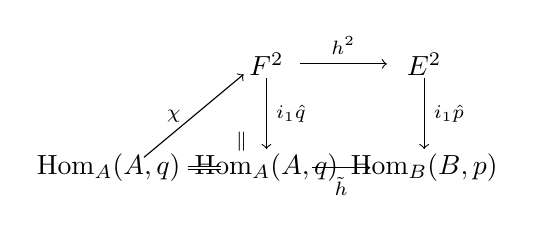
\begin{tikzpicture}[x=1.5em,y=1.5em]
  \node (HA1) at (0,-0.8) {$\mathrm{Hom}_{A}(A,q)$};
  \node (HA2) at (3.8,-0.8) {$\mathrm{Hom}_{A}(A,q)$};
  \node (HB) at (7.6,-0.8) {$\mathrm{Hom}_{B}(B,p)$};
  \node (F2) at (3.8,1.7) {$F^{2}$};
  \node (E2) at (7.6,1.7) {$E^{2}$};
  \draw[->] (4.6,1.7) -- node[above]{$\scriptstyle h^{2}$} (6.7,1.7);
  \draw[->] (3.8,1.35) -- node[right]{$\scriptstyle i_{1}\hat{q}$} (3.8,-0.35);
  \draw[->] (7.6,1.35) -- node[right]{$\scriptstyle i_{1}\hat{p}$} (7.6,-0.35);
  \draw[double] (1.9,-0.8) -- (2.7,-0.8);
  \draw[->] (4.9,-0.8) -- node[below]{$\scriptstyle\tilde{h}$} (6.3,-0.8);
  \draw[->] (0.85,-0.55) -- node[above,pos=0.3]{$\scriptstyle\qcor{\chi}$} (3.25,1.45);
  \node at (3.2,-0.18) {$\scriptstyle\parallel$};
\end{tikzpicture}
\end{center}
由附录 B 中的定义 B.3.3，这一方块经由 $i_{1}\hat{p}\dashv\qcor{\chi}$ 的余单位%
$\bar{\eta}$ 的一个须化副本 $\bar{\eta}h^{2}\qcor{\chi}$，穿过下方偏右所展示的%
那个绝对右提升图表而分解：

\begin{center}
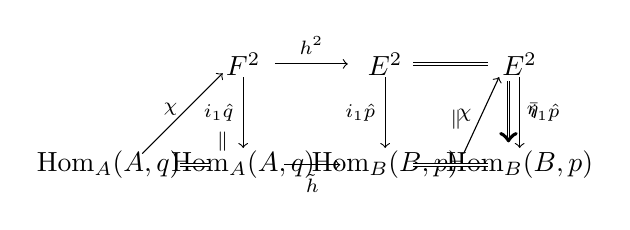
\begin{tikzpicture}[x=1.35em,y=1.35em]
  \node (HA1) at (0,-0.9) {$\mathrm{Hom}_{A}(A,q)$};
  \node (HA2) at (3.6,-0.9) {$\mathrm{Hom}_{A}(A,q)$};
  \node (HB1) at (7.4,-0.9) {$\mathrm{Hom}_{B}(B,p)$};
  \node (HB2) at (11.0,-0.9) {$\mathrm{Hom}_{B}(B,p)$};
  \node (F2) at (3.6,1.8) {$F^{2}$};
  \node (E2a) at (7.4,1.8) {$E^{2}$};
  \node (E2b) at (11.0,1.8) {$E^{2}$};
  \draw[->] (4.45,1.8) -- node[above]{$\scriptstyle h^{2}$} (6.4,1.8);
  \draw[double] (8.15,1.8) -- (10.15,1.8);
  \draw[double] (1.9,-0.9) -- (2.7,-0.9);
  \draw[->] (4.7,-0.9) -- node[below]{$\scriptstyle\tilde{h}$} (6.2,-0.9);
  \draw[double] (8.15,-0.9) -- (10.15,-0.9);
  \draw[->] (3.6,1.45) -- node[left]{$\scriptstyle i_{1}\hat{q}$} (3.6,-0.45);
  \draw[->] (7.4,1.45) -- node[left]{$\scriptstyle i_{1}\hat{p}$} (7.4,-0.45);
  \draw[->] (11.0,1.45) -- node[right]{$\scriptstyle i_{1}\hat{p}$} (11.0,-0.45);
  \draw[->] (0.9,-0.6) -- node[above,pos=0.35]{$\scriptstyle\qcor{\chi}$} (3.05,1.55);
  \node at (3.05,-0.28) {$\scriptstyle\parallel$};
  \draw[->] (9.5,-0.6) -- node[left]{$\scriptstyle\qcor{\chi}$} (10.45,1.45);
  \node at (9.3,0.3) {$\scriptstyle\parallel$};
  \draw[double,->] (10.7,1.35) -- (10.7,-0.3);
  \node at (11.35,0.55) {$\scriptstyle\bar{\eta}$};
\end{tikzpicture}
\end{center}
于是，由\cref{thm:pcartesian-characterizations}(ii)，$\bar{\eta}h^{2}\qcor{\chi}$ %
可逆，当且仅当 $h^{2}\qcor{\chi}$ 是 $p$-\trCartesian。

\textbf{(i)$\Leftrightarrow$(iii)：}由于 $\Delta_{p}\dashv r$ 的单位是同构——%
其理由已在定理 5.2.8(iii) 的陈述中讨论过——(iii) 左侧那个同构的对应便同构于%
$r\tilde{h}\epsilon$，于是我们的任务是证明：这一\trNaturalTransformation{} %
可逆，当且仅当 $h$ 定义一个笛卡尔函子。
这就引导我们考虑表达两个余单位之水平复合的须化自然性方块：
\begin{center}
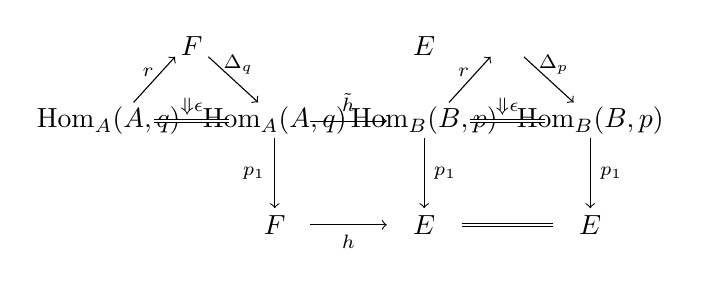
\begin{tikzpicture}[x=1.5em,y=1.5em]
  \node (Fq) at (2.0,2.7) {$F$};
  \node (Ep) at (7.6,2.7) {$E$};
  \node (HA1) at (0,0.9) {$\mathrm{Hom}_{A}(A,q)$};
  \node (HA2) at (4.0,0.9) {$\mathrm{Hom}_{A}(A,q)$};
  \node (HB1) at (7.6,0.9) {$\mathrm{Hom}_{B}(B,p)$};
  \node (HB2) at (11.6,0.9) {$\mathrm{Hom}_{B}(B,p)$};
  \node (Fb) at (4.0,-1.6) {$F$};
  \node (Eb1) at (7.6,-1.6) {$E$};
  \node (Eb2) at (11.6,-1.6) {$E$};
  \draw[->] (0.6,1.35) -- node[above,pos=0.35]{$\scriptstyle r$} (1.6,2.45);
  \draw[->] (2.4,2.45) -- node[above,pos=0.6]{$\scriptstyle\Delta_{q}$} (3.6,1.35);
  \draw[double] (1.1,0.9) -- (2.9,0.9);
  \node at (2.0,1.24) {$\scriptstyle\Downarrow\epsilon$};
  \draw[->] (8.2,1.35) -- node[above,pos=0.35]{$\scriptstyle r$} (9.2,2.45);
  \draw[->] (10.0,2.45) -- node[above,pos=0.6]{$\scriptstyle\Delta_{p}$} (11.2,1.35);
  \draw[double] (8.7,0.9) -- (10.5,0.9);
  \node at (9.6,1.24) {$\scriptstyle\Downarrow\epsilon$};
  \draw[->] (4.85,0.9) -- node[above]{$\scriptstyle\tilde{h}$} (6.7,0.9);
  \draw[->] (4.85,-1.6) -- node[below]{$\scriptstyle h$} (6.7,-1.6);
  \draw[double] (8.5,-1.6) -- (10.7,-1.6);
  \draw[->] (4.0,0.5) -- node[left]{$\scriptstyle p_{1}$} (4.0,-1.2);
  \draw[->] (7.6,0.5) -- node[right]{$\scriptstyle p_{1}$} (7.6,-1.2);
  \draw[->] (11.6,0.5) -- node[right]{$\scriptstyle p_{1}$} (11.6,-1.2);
\end{tikzpicture}
\end{center}
\begin{center}
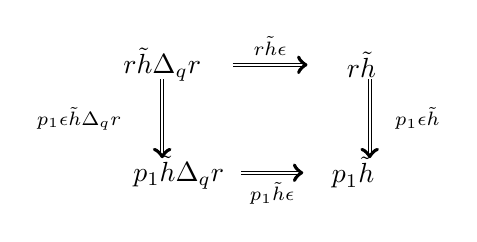
\begin{tikzpicture}[x=1.5em,y=1.5em]
  \node (TL) at (0,1.5) {$r\tilde{h}\Delta_{q}r$};
  \node (TR) at (4.8,1.5) {$r\tilde{h}$};
  \node (BL) at (0.4,-1.1) {$p_{1}\tilde{h}\Delta_{q}r$};
  \node (BR) at (4.6,-1.1) {$p_{1}\tilde{h}$};
  \draw[double,->] (1.7,1.5) -- node[above]{$\scriptstyle r\tilde{h}\epsilon$} (3.5,1.5);
  \draw[double,->] (1.9,-1.1) -- node[below]{$\scriptstyle p_{1}\tilde{h}\epsilon$} (3.4,-1.1);
  \draw[double,->] (0,1.15) -- (0,-0.75);
  \node at (-2.0,0.2) {$\scriptstyle p_{1}\epsilon\tilde{h}\Delta_{q}r$};
  \draw[double,->] (5.0,1.15) -- (5.0,-0.75);
  \node at (6.15,0.2) {$\scriptstyle p_{1}\epsilon\tilde{h}$};
\end{tikzpicture}
\end{center}
由于 $\epsilon$ 是伴随 $\Delta_{p}\dashv r$ 的余单位而该伴随的单位可逆，%
$\epsilon\Delta_{p}$ 是一个同构，于是 $\epsilon\tilde{h}\Delta_{q}=\epsilon\Delta_{p}h$ %
可逆。由计算 $pr\tilde{h}\epsilon=p_{0}\tilde{h}\epsilon=kp_{0}\epsilon=\mathrm{id}$ %
可见：顶部的水平 2-胞腔落在恒同之上的一个纤维中。

回忆定理 5.2.8(iii)：$p_{1}\epsilon$ 为笛卡尔纤维化 $p\colon E\twoheadrightarrow B$ %
定义了引理 5.2.5 中的那个泛 $p$-笛卡尔提升。
于是，右侧竖直 2-胞腔 $p_{1}\epsilon\tilde{h}$ 是 $\phi\tilde{h}$ 的一个 $p$-笛卡尔%
提升，其中 $\phi$ 是 $p$ 之上的右逗号锥。
由 $\tilde{h}$ 的定义，$\phi\tilde{h}=k\phi$，此处后一个 $\phi$ 是 $q$ 之上的%
右逗号锥。

类似地，底部的水平 2-胞腔 $p_{1}\tilde{h}\epsilon$ 是 $k\phi=\phi\tilde{h}$ 的一个%
提升。于是，若 $h$ 是一个笛卡尔函子，则右侧竖直与底部水平这两个 2-胞腔便是公共%
2-胞腔的两个 $p$-笛卡尔提升，从而\cref{lem:cartesian-conservativity}的保守性性质%
蕴含 $r\tilde{h}\epsilon$ 可逆。反之，若 $r\tilde{h}\epsilon$ 可逆，%
则 $p_{1}\tilde{h}\epsilon=hp_{1}\epsilon$ 同构于 $p$-笛卡尔变换 $p_{1}\epsilon\tilde{h}$，%
从而是 $p$-笛卡尔的。由于每个 $q$-笛卡尔变换都同构于 $p_{1}\epsilon$ 的一个限制，%
此情形成立当且仅当 $h$ 是一个笛卡尔函子。
\end{proof}

定理 5.2.8 与\cref{thm:cartesian-functor-characterization}的众多应用之一是：

\begin{corollary}\label{cor:cosmological-functors-preserve-cartesian}
\trCosmologicalFunctor{}保持\trCartesianArrow、\trCartesianFibration{}与笛卡尔函子。
\end{corollary}

\begin{proof}
由定理 5.2.8(ii)，$\infty$-宇宙 $\mathcal{K}$ 中的一条\trIsofibration{} %
$p\colon E\twoheadrightarrow B$ 是\trCartesian，当且仅当\trIsofibration{} %
$i_{1}\hat{p}\colon E^{2}\twoheadrightarrow\mathrm{Hom}_{B}(B,p)$ 容许一个右伴随%
右逆。\trCosmologicalFunctor{} $F\colon\mathcal{K}\to\mathcal{L}$ 保持%
\trIsofibration{}类以及定义这一映射 $i_{1}\hat{p}$ 的诸单纯极限。
由于与\trCosmologicalFunctor{}相关联的\trTwoFunctor{} %
$F\colon\mathfrak{h}\mathcal{K}\to\mathfrak{h}\mathcal{L}$ 保持伴随与 2-胞腔的%
可逆性，$F$ 保持\trCartesianFibration。笛卡尔函子的保持性类似地由%
\cref{thm:cartesian-functor-characterization}(ii) 得出。由推论 3.5.7，%
\trCosmologicalFunctor{}保持绝对右提升图表，故\trCartesianArrow{}的保持性由%
\cref{thm:pcartesian-characterizations}(ii) 得出。
\end{proof}

笛卡尔函子的另一族例子由下面这条引理给出，它可以用%
\cref{thm:cartesian-functor-characterization}来证明。

\begin{lemma}\label{lem:fibered-right-adjoint}
一个纤维化右伴随函子在具有公共底的\trCartesianFibration{}之间定义一个笛卡尔函子：
\begin{center}
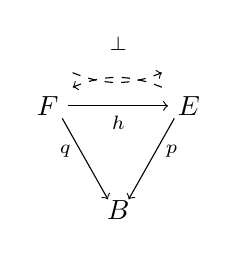
\begin{tikzpicture}[x=1.5em,y=1.5em]
  \node (F) at (0,1.4) {$F$};
  \node (E) at (3.4,1.4) {$E$};
  \node (B) at (1.7,-1.1) {$B$};
  \draw[->,dashed] (2.75,1.85) to[bend right=22] (0.6,1.85);
  \draw[->,dashed] (0.6,2.2) to[bend right=22] (2.75,2.2);
  \node at (1.7,2.9) {$\scriptstyle\bot$};
  \draw[->] (0.5,1.4) -- node[below]{$\scriptstyle h$} (2.9,1.4);
  \draw[->] (0.35,1.1) -- node[left,pos=0.4]{$\scriptstyle q$} (1.45,-0.85);
  \draw[->] (3.05,1.1) -- node[right,pos=0.4]{$\scriptstyle p$} (1.95,-0.85);
\end{tikzpicture}
\end{center}
\end{lemma}

\begin{proof}
设 $\ell$ 在 $\infty$-宇宙 $\mathcal{K}$ 中是 $h$ 的一个纤维化左伴随，则由拉回%
定义的\trCosmologicalFunctor{} $p_{1}^{*}\colon\mathcal{K}_{/B}\to\mathcal{K}_{/B^{2}}$ %
把这一\trFiberedAdjunction{}送到\trFiberedAdjunction
\begin{center}
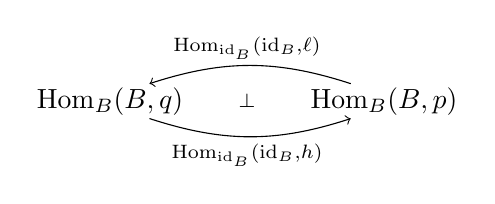
\begin{tikzpicture}[x=1.5em,y=1.5em]
  \node (HA) at (0,0) {$\mathrm{Hom}_{B}(B,q)$};
  \node (HB) at (6.6,0) {$\mathrm{Hom}_{B}(B,p)$};
  \draw[->] (5.8,0.42) to[bend right=18] (0.95,0.42);
  \node at (3.3,1.28) {$\scriptstyle\mathrm{Hom}_{\mathrm{id}_{B}}(\mathrm{id}_{B},\ell)$};
  \draw[->] (0.95,-0.42) to[bend right=18] (5.8,-0.42);
  \node at (3.3,-1.3) {$\scriptstyle\mathrm{Hom}_{\mathrm{id}_{B}}(\mathrm{id}_{B},h)$};
  \node at (3.3,0) {$\scriptstyle\bot$};
\end{tikzpicture}
\end{center}
类似地，\trCosmologicalFunctor{} $(-)^{2}\colon\mathcal{K}\to\mathcal{K}$ 把伴随%
$\ell\dashv h$ 送到伴随 $\ell^{2}\dashv h^{2}$。

现在，交换方块
\begin{center}
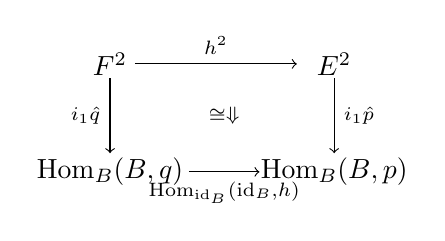
\begin{tikzpicture}[x=1.5em,y=1.5em]
  \node (F2) at (0,1.6) {$F^{2}$};
  \node (E2) at (5.4,1.6) {$E^{2}$};
  \node (HA) at (0,-1.0) {$\mathrm{Hom}_{B}(B,q)$};
  \node (HB) at (5.4,-1.0) {$\mathrm{Hom}_{B}(B,p)$};
  \draw[->] (0.6,1.6) -- node[above]{$\scriptstyle h^{2}$} (4.5,1.6);
  \draw[->] (0,1.25) -- node[left]{$\scriptstyle i_{1}\hat{q}$} (0,-0.55);
  \draw[->] (5.4,1.25) -- node[right]{$\scriptstyle i_{1}\hat{p}$} (5.4,-0.55);
  \draw[->] (1.9,-1.0) -- node[below]{$\scriptstyle\mathrm{Hom}_{\mathrm{id}_{B}}(\mathrm{id}_{B},h)$} (3.6,-1.0);
  \node at (2.75,0.35) {$\scriptstyle\cong\Downarrow$};
\end{tikzpicture}
\end{center}
中的两个水平函子都容许左伴随。对应演算中的一个标准结果告诉我们：关于竖直伴随的%
对应是一个同构，当且仅当关于水平伴随的对应是一个同构；后者这一诸左伴随之间的%
\trNaturalTransformation{}正是前者这一诸右伴随之间的\trNaturalTransformation{} %
的转置（见练习 B.3.iii）。在当前语境下，借助 $\mathrm{Hom}_{B}(B,q)$ 的%
\trTwoCellConservativity{}即可看出：关于水平伴随的对应是一个同构。
\end{proof}

\subsection*{练习}

\begin{exercise}\label{ex:pullback-of-cartesian-functor}
证明：具有公共底的\trCartesianFibration{}之间的一个笛卡尔函子 $h$ 的%
\trPullback{}定义一个笛卡尔函子
\begin{center}
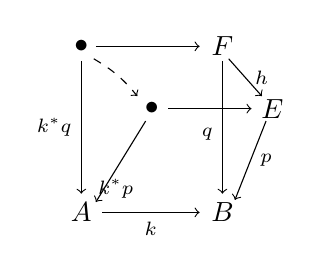
\begin{tikzpicture}[x=1.5em,y=1.5em]
  \node (P) at (0,3.0) {$\bullet$};
  \node (F) at (3.4,3.0) {$F$};
  \node (Q) at (1.7,1.5) {$\bullet$};
  \node (E) at (4.6,1.5) {$E$};
  \node (A) at (0,-1.0) {$A$};
  \node (B) at (3.4,-1.0) {$B$};
  \draw[->] (0.35,3.0) -- (2.85,3.0);
  \draw[->,dashed] (0.3,2.7) to[bend left=10] (1.35,1.8);
  \draw[->] (2.1,1.5) -- (4.1,1.5);
  \draw[->] (3.55,2.7) -- node[right]{$\scriptstyle h$} (4.35,1.8);
  \draw[->] (3.4,2.65) -- node[left,pos=0.55]{$\scriptstyle q$} (3.4,-0.55);
  \draw[->] (4.45,1.2) -- node[right,pos=0.5]{$\scriptstyle p$} (3.7,-0.7);
  \draw[->] (0,2.65) -- node[left]{$\scriptstyle k^{*}q$} (0,-0.55);
  \draw[->] (1.55,1.2) -- node[below,pos=0.6]{$\scriptstyle k^{*}p$} (0.35,-0.75);
  \node at (2.02,1.16) {$\scriptstyle\llcorner$};
  \draw[->] (0.5,-1.0) -- node[below]{$\scriptstyle k$} (2.85,-1.0);
\end{tikzpicture}
\end{center}
\end{exercise}

\begin{exercise}\label{ex:cartesian-functors-compose}
证明：笛卡尔函子既可沿竖直方向又可沿水平方向复合。
\end{exercise}

\begin{exercise}\label{ex:contravariant-bindexed-functors}
把「\trCartesianFibration{} $p\colon E\twoheadrightarrow B$ 与 $q\colon F\twoheadrightarrow B$ 定义了『取值于 $\infty$-范畴的反变 $B$-指标函子』」这一%
直觉加以范畴化：证明一个笛卡尔函子
\begin{center}
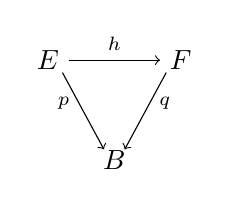
\begin{tikzpicture}[x=1.5em,y=1.5em]
  \node (E) at (0,1.4) {$E$};
  \node (F) at (3.2,1.4) {$F$};
  \node (B) at (1.6,-1.0) {$B$};
  \draw[->] (0.5,1.4) -- node[above]{$\scriptstyle h$} (2.7,1.4);
  \draw[->] (0.35,1.1) -- node[left,pos=0.4]{$\scriptstyle p$} (1.35,-0.75);
  \draw[->] (2.85,1.1) -- node[right,pos=0.4]{$\scriptstyle q$} (1.85,-0.75);
\end{tikzpicture}
\end{center}
定义了一个「自然变换」：证明在下述纤维方块中
\begin{center}
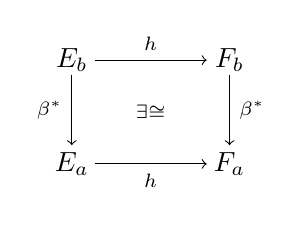
\begin{tikzpicture}[x=1.5em,y=1.5em]
  \node (Eb) at (0,1.5) {$E_{b}$};
  \node (Fb) at (3.8,1.5) {$F_{b}$};
  \node (Ea) at (0,-1.0) {$E_{a}$};
  \node (Fa) at (3.8,-1.0) {$F_{a}$};
  \draw[->] (0.55,1.5) -- node[above]{$\scriptstyle h$} (3.25,1.5);
  \draw[->] (0.55,-1.0) -- node[below]{$\scriptstyle h$} (3.25,-1.0);
  \draw[->] (0,1.15) -- node[left]{$\scriptstyle\beta^{*}$} (0,-0.55);
  \draw[->] (3.8,1.15) -- node[right]{$\scriptstyle\beta^{*}$} (3.8,-0.55);
  \node at (1.9,0.25) {$\scriptstyle\exists\cong$};
\end{tikzpicture}
\end{center}
存在一个自然同构，其中 $B$ 的\trHomotopyCategory{}中的一支箭头 $\beta$ 在诸%
纤维上的作用，定义为把 $\beta$ 的某个 $p$-或 $q$-笛卡尔提升的定义域作分解，%
如 (5.0.1) 所展示的那样。
\end{exercise}
